\chapter{OpenDQ operation}
\label{sec:06-operation}
This chapter describes the operation of the different protocols that are used in the OpenDQ project to enable distributed data collection using low-power wireless technologies. As a remainder, the operation of a data collection protocol is split into two different phases: synchronization and data transmission. In the synchronization phase the gateway uses a PS (Preamble Sampling) mechanism to wake-up and synchronize all the nodes that are within its communication range. In the data transmission phase the nodes that are synchronized use a MAC (Medium Access Control) protocol, i.e., FSA (Frame Slotted ALOHA) or DQ (Distributed Queuing), to transmit their data packets to the gateway. Finally, the gateway forwards the received data packets to the computer, where they are processed, stored and represented.

%%
% Overview
%%
\section{Overview}
To enable distributed data collection using low-power wireless technologies, the OpenDQ project defines the physical and the data-link layers of the OSI (Open Systems Interconnect) model.

At the physical layer the OpenDQ project uses the IEEE~802.15.4 standard \cite{ieee802.15.4-2006}, which operates at the 2.45~GHz ISM (Industrial, Scientific and Medic) band, which is available world-wide. At the 2.45~GHz band (2400-2483~MHz, 83~MHz), the IEEE~802.15.4 standard defines 16 channels (from 11 to 26) with a 2~MHz bandwidth and a channel separation of 5~MHz. The physical layer uses an OQPSK (Offset Quadrature Phase-Shift Keying) modulation with DSSS (Direct Sequence Spread Spectrum), which provides an effective data rate of 250~kbps, as depicted in Figure~\ref{fig:07-modulation}. For a complete description of the IEEE~802.15.4 standard please refer to the standard document \cite{ieee802.15.4-2006}.

% IEEE 802.15.4 physical layer modulation scheme
\begin{figure}[!ht]
    \centering
	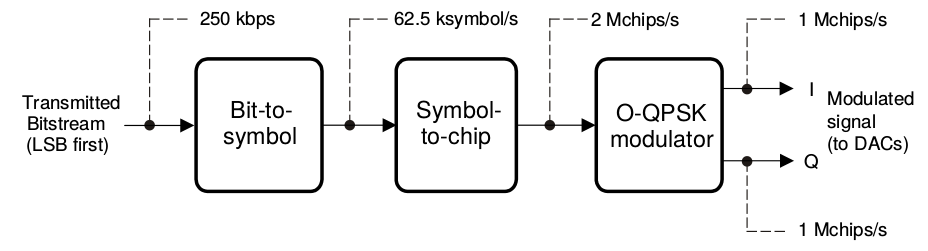
\includegraphics[width=0.75\linewidth]{07-modulation}
    \caption[IEEE 802.15.4 physical layer modulation scheme]{IEEE 802.15.4 physical layer modulation scheme. [Source: Texas Instruments]}
    \label{fig:07-modulation}
\end{figure}

At the physical layer the IEEE~802.15.4 standard also defines the PPDU (Physical Protocol Data Unit). The PPDU is composed of a SHR (Synchronization Header, 5 bytes), which is composed of a PS (Preamble Sequence, 4 bytes) and a SFD (Start-of-Frame Delimiter, 1 byte), a PHR (Physical Header, 1 byte) and the PSDU (Physical Service Data Unit), as depicted in Figure~\ref{fig:07-frame}. The PHR contains the number of payload bytes in the MPDU (MAC Protocol Data Unit), which is limited to 127~bytes and contains a 2-byte FCS (Frame-Check Sequence) that enables to check the integrity of the data payload.

% Schematic View of the IEEE 802.15.4 Frame Format
\begin{figure}[!it]
    \centering
	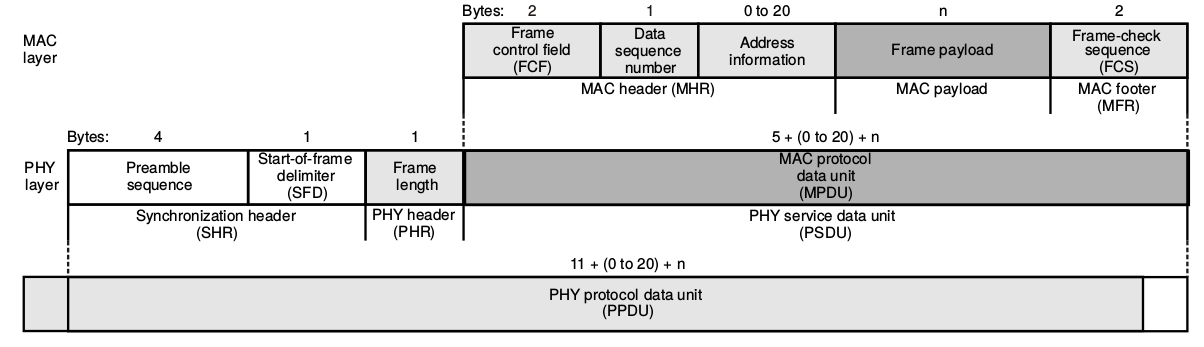
\includegraphics[width=0.75\linewidth]{07-frame}
    \caption[Schematic view of the IEEE 802.15.4 frame format]{Schematic view of the IEEE 802.15.4 frame format. [Source: Texas Instruments]}
    \label{fig:07-frame}
\end{figure}

At the data-link layer, OpenDQ provides the implementation of the data-link layer protocols that are required for the synchronization and the data transmit phases of data collection. In particular, it provides an implementation of a packet-based PS mechanism that is used by the gateway during the synchronization phase to wake-up all the nodes that are within its communication range. It also provides the implementation of two MAC protocols, i.e., FSA and DQ, that are used by nodes to transmit their data packets to the gateway during the data transmission phase. Despite having a different purpose, there are two common aspects of all data-link layer protocols implemented in the OpenDQ project, as described next.

First, the data-link layer protocols are implemented as finite-state machines, where the future state of the system depends on the current state, as well as time progress and external events. To implement the finite-state machine of each protocol the states are defined and each state is implemented as a C function. Typically, each state is split into \textit{init} and \textit{done} functions to indicate its entry and exit points, but states can also have sub-states. Each C function carries all the tasks that are required in the current state, i.e., prepare a packet and turn on the radio transceiver to transmit it, and prepares the system to evolve to the next state, i.e., obtain a packet handler and turn on the radio transceiver to receive a packet. Thus, the advance from a state to the next state can be triggered by synchronous or asynchronous events. For example, a timer that expires would be a synchronous event, whereas a packet being received would be an asynchronous event.

Second, the data-link layer protocols require time synchronization between the gateway and the nodes that are within its communication range to be able to wake-up and exchange data. In order to achieve such distributed synchronization a common time unit is defined. The tick is defined as $1/32.768$~Hz, which translates into $30.51$~us, and is derived from the RTC (Real-Time Clock) that each device has. One important aspect to take into account for the protocol implementation is that the RTC drift. That is, due to the physical construction limitations of crystals and environmental effects, i.e., temperature, the tick rate of RTCs change along time. For instance, the RTC clocks that are used on the OpenMote-CC2538 board have a nominal drift rate of 20~ppm. This implies that two devices of the network can drift up to $\pm$40~ppm, one crystal going fast and the other going slow. This has several implication in the design of the data-link layer protocols since mechanisms to compensate for such drift are required to ensure proper operation of the network.

The operation of WOR for the synchronization phase, as well FSA and DQ for the data transmission phase, are explained in detail in the next subsections.

%%
% Wake-on Radio
%%
\section{Wake-On Radio}
\label{sec:06-wor}
WOR (Wake-On Radio), depicted in Figure~\ref{fig:07-wor}, is the module that implements the packet-based PS (Preamble Sampling) mechanism that is used in the synchronization phase to allow the gateway wake-up all the nodes that are within its communication range and provide the information required for the data transmission phase. In particular, the WOR mechanism determines the time and channel at which nodes are expected to wake up to start the data transmission phase, as well as the MAC layer that they are expected to execute, i.e., DQ or FSA, to transmit their data packets to the gateway.

% Wake on Radio operation
\begin{figure}[!ht]
    \centering
	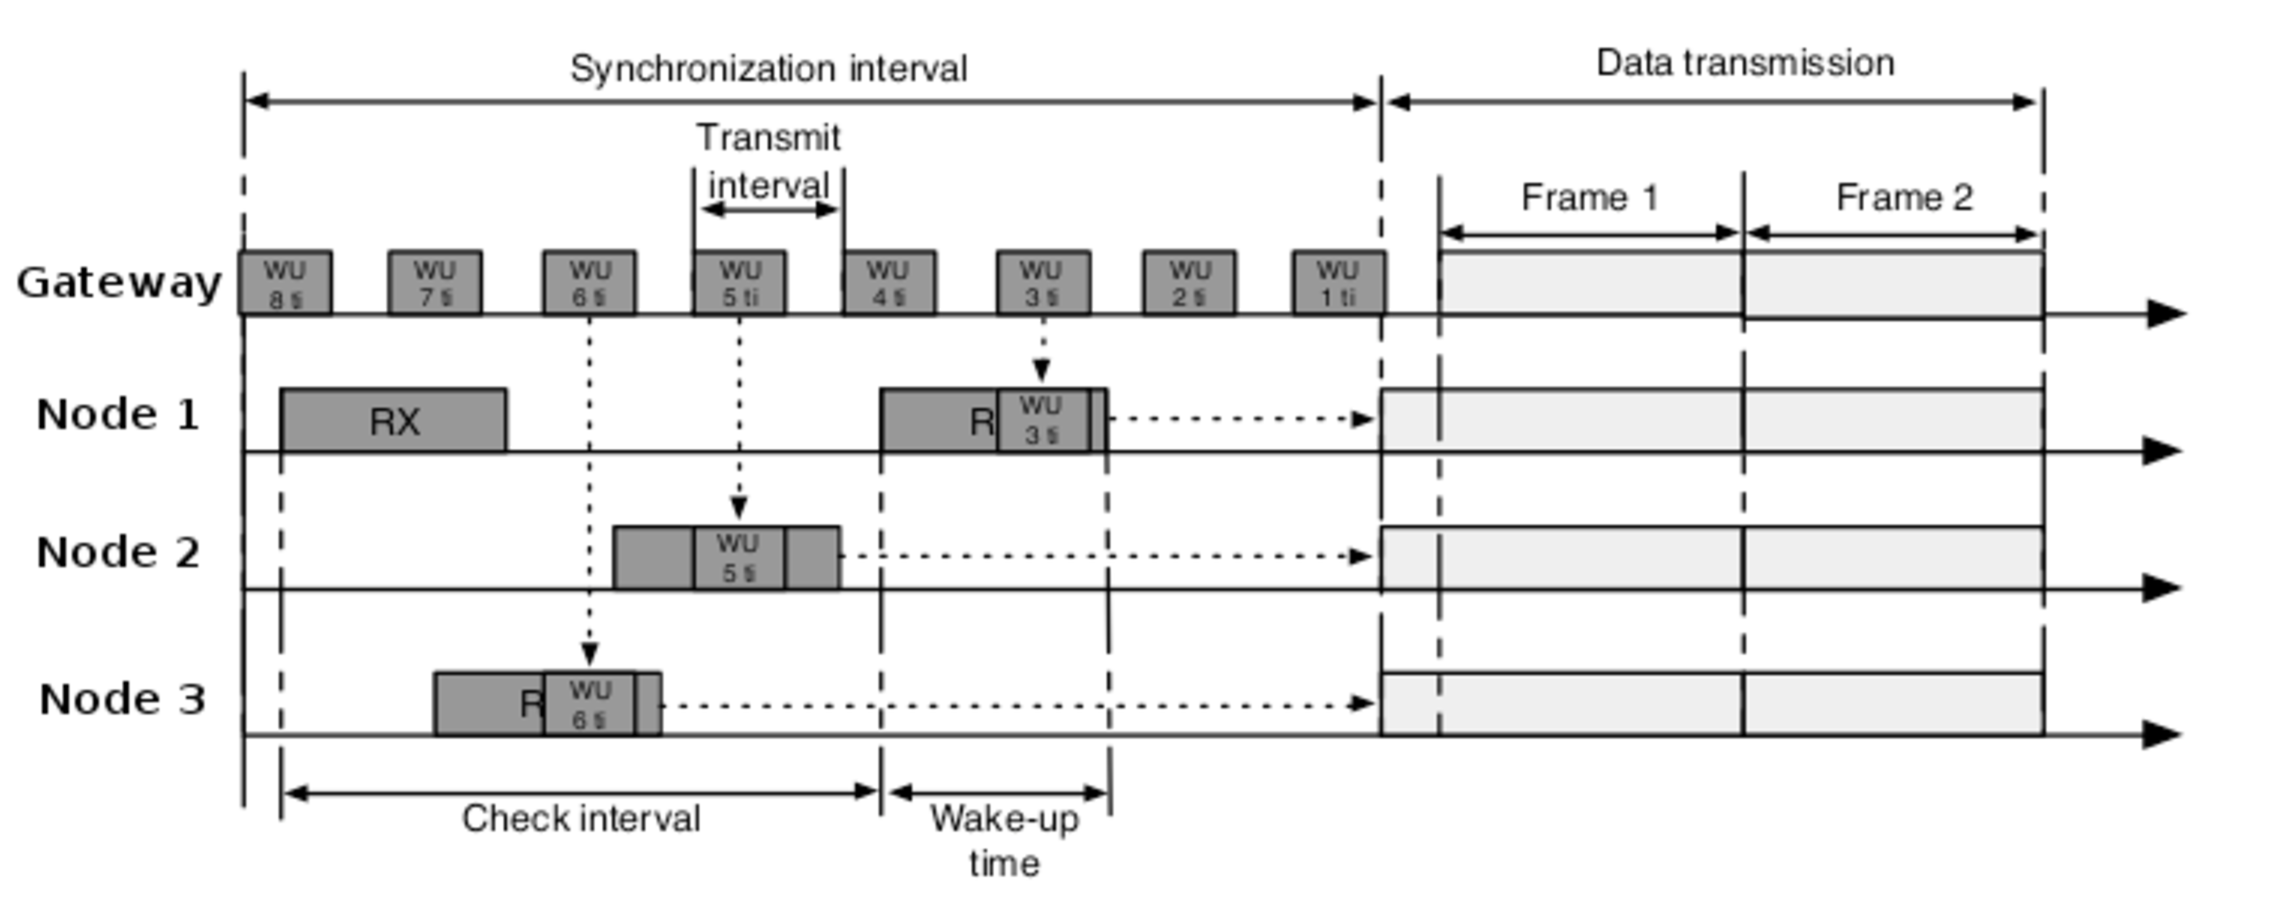
\includegraphics[width=0.75\linewidth]{07-wor}
    \caption{Wake-On Radio operation.}
    \label{fig:07-wor}
\end{figure}

The WOR mechanism that is implemented in the OpenDQ project can be found in the $wor.c$ and $wor.h$ files under the $protocols$ folder. The implementation of WOR contains two different flavours, one for the gateway and for the node, which are selected at compile time using a macro defined in the project configuration file ($config.h$).

The WOR implementation for the gateway is responsible to transmit the wake-up packets that enable the nodes and wake-up at the appropriate time to start the data collection phase. The main parameters of the WOR gateway implementation are the transmit duration, the transmit period and the number of packets, as summarized in Table~\ref{tab:06-wor}. The transmit duration indicates how long does the gateway keep sending WOR packets in order to wake-up nodes, whereas the transmit period indicates how often does the gateway transmit such WOR packets. The number of packets transmitted in a period results from dividing the transmit duration by the transmit period. By default the transmit duration is 65536~ticks (2~seconds) and the transmit period is 32~ticks (976,32~us), which means that the gateway will transmit a total of 2048~packets, one every 976,32~us. Considering the physical layer data rate, i.e., 250~kbps, and length of a WOR packet, i.e., 13~bytes including the SHR, it takes 416~us to transmit a WOR packet. Thus, the transmit duty cycle of the gateway when transmitting the synchronization packets is around 50\%.

In turn, the WOR implementation for the node is responsible to periodically turn on the radio transceiver to try to receive a WOR packet from the gateway to wake-up. The main parameters of the node implementation are the receive period and the receive duration, as summarized in Table~\ref{tab:06-wor}. The receive period indicates how often does the system turn on the radio to try to receive a WOR packet from the gateway, whereas the receive duration indicates how long does the system keep the radio on to receive a WOR packet from the gateway. By default the receive period is 32768~ticks (1~second) and the receive duration is 64~ticks (1952~us), which translates into a radio duty cycle of 0.2\%. It is important to notice that such values have been selected to ensure that any node will receive at least one WOR packet from the gateway regardless of its wake-up duty cycle. The values selected for the gateway and node are a good compromise between wake-up delay and energy consumption. However, it is possible to adjust such values to improve wake-up delay at the expense of increasing the energy consumption of the nodes.

% Wake-on Radio configuration parameters
\begin{table}[!it]
\centering
\begin{tabular}{|c|c|c|}
\hline
\textbf{PARAMETER} & \textbf{VALUE} \\ \hline
$WOR\_TX\_DURATION$  & 65536 ticks    \\ \hline
$WOR\_TX\_PERIOD$    & 32 ticks       \\ \hline
$WOR\_TX\_PACKETS$   & 2048 packets   \\ \hline
$WOR\_RX\_PERIOD$    & 32768 ticks    \\ \hline
$WOR\_RX\_DURATION$  & 64 ticks       \\
\hline
\end{tabular}
\label{tab:06-wor}
\caption{Wake-On Radio configuration parameters.}
\end{table}

In addition to the timing parameters, the WOR implementation also determines the WOR packet structure. Upon being triggered by the computer, the WOR packet is sent by the gateway periodically and contains the information required to synchronize the nodes. The WOR packet is then received by the node to configure the parameters of the data transmission phase. The WOR packet structure is defined in $wor\_packet\_t$ (in $wor.c$) and has a payload of 5~bytes with the following structure. However, notice that the payload of the $wor\_packet$ (5~bytes) will include the SHR (5~bytes) and the PHR (1~byte) at the beginning and the FCS (2~bytes) at the end, meaning that the whole $wor\_packet$ will have 13~bytes when transmitted by the radio transceiver. Also, notice that the $wor\_packet\_t$ is \textit{packed} to ensure that the compiler generates the appropriate data structure, i.e., without padding, since the structure is meant to be sent and received using the radio transceiver.
\begin{itemize}
\item $MAC\_TYPE$ [1 byte]. Indicates the MAC type, i.e., DQ or FSA, to be executed by Nodes in the data transmission phase.
\item $MAC\_PACKET$ [1 byte]. Indicates the MAC packet, i.e. WOR, ARP, FBP, DATA and ACK. For WOR the packet type is always WOR.
\item $MAC\_TIME$ [2 bytes]. Indicates the time (in ticks) at which the nodes are expected to wake up to begin the data-transmit phase.
\item $MAC\_CHANNEL$ [1 byte]. Indicates the channel at which the nodes are expected to operate at the beginning of the data-transmit phase.
\end{itemize}

The WOR module also defines the $wor\_vars_t$ data structure to store the variables that are used during WOR execution for network synchronization. The implementation of both the gateway and the node require different variables during execution, but at the moment of writing this document both use the same data structure.
\begin{itemize}
\item $tx\_duration$. Used by the gateway to keep track of the WOR remaining duration until the beginning of the data transmission phase.
\item $tx\_period$. Used by the gateway to keep track of the WOR period.
\item $tx\_packets$. Used by the gateway to keep track of the remaining packets to be transmitted. When the remaining packet is zero the gateway starts the data transmission phase.
\item $rx\_period$. Used by the node to store the period of the WOR cycle.
\item $rx\_duration$. Used by the node to store the duration of each idle listening cycle.
\item $wor\_cb$. Used by the node to store the callback to the appropriate MAC for the data transmission phase, i.e., FSA or DQ.
\item $wor\_channel$. Used by the node to store the channel for the data transmission phase.
\end{itemize}

The WOR module also defines the following public functions that are common for both the gateway and the node implementation.
\begin{itemize}
\item $wor\_init$. Initializes the $wor_vars$ data structure. Called from the MAC module $mac\_init$ function during the initialization phase.
\item $wor\_set\_cb$. Registers a callback to the function that needs to be executed when the WOR finalizes and the data transmission phase begins. Typically it points to $mac\_start$, which is responsible to start the appropriate MAC protocol based on the information received in the WOR packet.
\item $wor\_cancel\_cb$. De-registers a callback to the function that needs to be executed when the WOR finalizes. Currently the function is not used.
\end{itemize}

The WOR module also defines the following private functions for the gateway implementation. As it is possible to observe, the gateway will transmit a given number of WOR packets (as determined by the parameters described above) and after that it will begin the execution of the appropriate MAC protocol, i.e., FSA or DQ. 
\begin{itemize}
\item $wor\_config$. Prepares to start the execution of the packet-based PS mechanism for the gateway by setting the appropriate values in the $wor\_vars$ and $mac\_vars$ data structures and pushing the $wor\_start$ task to the scheduler.
\item $wor\_start$. Prepares the $wor\_packet$ that will be transmitted to wake-up the nodes. It also turns on the radio transceiver, configures the radio channel and the transmit callbacks, and enables radio interrupts. After that, it copies the $wor\_packet$ to the radio transceiver and begins the transmission. Finally, it sets a time-out using the virtual timer module to indicate that the current transmit period has finished.
\item $wor\_tx\_init$. Callback from the radio transceiver to indicate that a packet is now being transmitted.
\item $wor\_tx\_done$. Callback from the radio transceiver to indicate that a packet has been successfully transmitted.
\item $wor\_done$. Callback from the virtual timer module that indicates that the current transmit period has finished. It turns off the radio and clears the callbacks, releases the packet buffer, and updates the WOR status. Finally, it decides the next action to take. If no more WOR packets need to be transmitted, it sets a time-out using the virtual timer module to start the data transmission phase with the appropriate MAC protocol. If more WOR packets need to be transmitted, it sets a time-out using the virtual timer module to start a new period using the $wor\_start$ function.
\end{itemize}

Similarly, the WOR module defines the following private functions for the node implementation. As it is possible to observe, the node will try to receive a WOR packet indefinitely by cycling between the $wor\_start$ and $wor\_timeout$ functions at the appropriate times. When a WOR packet is successfully received, the cycle will break and the node will progress to the $wor\_done$ function, where it will prepare for the execution of the MAC protocol according to the parameters set by the WOR packet transmitted by the gateway.
\begin{itemize}
\item $wor\_config$. Prepares to start the execution of the packet-based PS mechanism for the node by setting the appropriate values in the $wor\_vars$ data structure and pushing the $wor\_start$ task to the scheduler.
\item $wor\_start$. Starts the execution of the packet-based PS mechanism. It registers the radio callbacks, obtains a $packet\_buffer$ entry, turns on the radio in receive mode and sets a time-out for the $wor\_timeout$ function using the $virtual\_timer$ module in case no WOR packet is received.
\item $wor\_rx\_init$. Callback from the radio transceiver module that indicates that a packet has started to be received.
\item $wor\_rx\_done$. Callback from the radio transceiver module that indicates that a packet has finished being received. If a packet is successfully received it processes the packet. If it is a valid WOR packet it updates the $mac\_vars$ data structure with the MAC protocol, timing and channel information. Finally, it turns off the radio transceiver.
\item $wor\_timeout$. Callback from the virtual timer module that indicates that the current interval has expired. If a valid WOR packet has been received it prepares for the beginning of the data transmission phase by pushing the $wor\_done$ task to the $virtual\_timer$ to be executed at the appropriate time. If a valid WOR packet has not been received it prepares for the beginning of a new cycle by pushing the $wor\_start$ task to the $virtual\_timer$ to be executed at the appropriate time.
\item $wor\_done$. Releases the $packet\_buffer$ entry obtained in the $wor\_start$ function and schedules the start of the data transmission phase by pushing the $wor\_vars.wor\_cb$ task to the $virtual\_timer$ to be executed at the appropriate time. The $wor\_vars.wor\_cb$ will contain a function to the appropriate entry point for the MAC protocol to be executed in the data transmission phase, i.e., $fsa\_start$ or $dq\_start$.
\end{itemize}

%%
% Medium Access Control
%%
\section{Medium Access Control}
\label{sec:06-mac}
The MAC (Medium Access Control) is a module that provides the basic functionality to control the operation of the various MAC protocols implemented in the OpenDQ project for the data transmission phase, i.e., FSA and DQ. The implementation of the MAC module contains a single flavour that is common for both the gateway and for the node. However, the configuration of the MAC module to be used in the data transmission phase is filled in differently depending on the device type, i.e., gateway or node. In case the device is a gateway, the configuration is filled in through the serial port. Contrarily, if the device is a node, the configuration is filled in through the WOR mechanism during the synchronization phase.

The MAC module that is implemented in the OpenDQ project can be found in the $mac.c$ and $mac.h$ files under the $protocols$ folder. In particular, the MAC module provides the data structures, functions and variables to set the time at which the data transmission phase is expected to begin and also the protocol that the device is expected to execute. 

The MAC module defines the following data types that are common for all MAC protocols. This data types are used instead of the raw values to enforce type checking in function calls.
\begin{itemize}
\item $mac\_address\_t$ [$uint16\_t$]. Used by the gateway or the nodes to determine the device that originates or has to receive a given packet. The 16-bit address is derived from the EUI-64 address by taking the least two significant bytes. There are also two values that are reserved: invalid ($0x0000$) and broadcast ($0xFFFF$) as defined in $mac\_addr\_type\_t$.
\item $mac\_seq\_number\_t$ [$uint16\_t$]. Incremental sequence number that is used by nodes to ensure that they are synchronized with the gateway. If a node receives a packet that does not contain a valid sequence number it can assume that it has lost synchronization with the gateway and trigger the appropriate action, i.e., reset the value or reset itself.
\item $mac\_time\_t$ [$uint16\_t$]. Time at which a certain event is expected to happen at the MAC layer. Each LSB is equivalent to one tick of the RTC ($30.51$~us). Since the counter is only 16-bit wide it wraps around after 65535~ticks or 2~seconds.
\item $mac\_channel\_t$ [$uint8\_t$]. Channel of the IEEE~802.15.4 physical layer, i.e., between 11 and 26, at which the data transmission phase will begin. After that the channel of each transmission can change if channel hopping is enabled.
\item $mac\_slots\_t$ [$uint8\_t$]. Number of slots. For FSA the number of slots indicates the number of slots per frame, whereas for DQ the number of slots per frame can be used to indicate the number of ARP slots in the access sub-period.
\end{itemize}

The MAC module defines the following data structures that are common for all MAC protocols.
\begin{itemize}
\item $mac\_state\_t$. Indicates if the MAC is synchronized or unsynchronized. The MAC can be in two possible states, unsynchronized ($0x00$) or synchronized ($0x01$). If the MAC is synchronized the synchronization LED (orange) will be turned on. IF the MAC is not synchronized the synchronization LED (orange) will be turned off.
\item $mac\_type\_t$. Defines the MAC types that are supported. Currently the protocols implemented are FSA ($0x01$) and DQ ($0x02$). The gateway receives this value as a parameter from the computer and uses it in the synchronization phase using WOR to announce the type of MAC protocol that will be executed in the data transmission phase. Nodes receive this value as a parameter during the synchronization phase using WOR and use it to start the appropriate MAC protocol in the data transmission phase.
\item $mac\_packet\_t$. Indicates the type of packet that is being transmitted or that has to be received. Currently there are five types of packets which are used by the different protocols. The packet types are WOR ($0x01$), ARP ($0x02$), FBP ($0x03$), DATA ($0x04$) and ACK ($0x05$). The WOR implementation only uses the WOR packet type. The FSA implementation uses the FBP, DATA and ACK. Finally, the DQ implementation uses the ARP, FBP and DATA.
\item $mac\_packet\_state\_t$. Indicates the status of a packet. Currently a packet, either a DATA or ACK packet, can be in three different states, empty ($0x00$), error ($0x01$) or success ($0x02$). Empty is used when the energy level in the channel is below a given threshold and no packet has been detected. Error is used when the energy level in the channel is above a given threshold but a packet has not been successfully received. Finally, success indicates that a packet has been successfully received.
\item $mac\_rssi\_state\_t$. Indicate the RSSI (Received Signal Strength Indicator) status of a packet. Currently, the RSSI status of a packet can be in three states, none ($0x00$), below ($0x01$) or above ($0x02$). None indicates that the RSSI was not sensed, below indicates that is below a given threshold and, finally, above indicates that it is above a given threshold. The RSSI threshold is defined in each implementation in a macro named $FSA\_RSSI\_THRESHOLD$ or $DQ\_RSSI\_THRESHOLD$ depending on the protocol.
\end{itemize}

The MAC module defines the following public functions. This function are meant to be called from outside the MAC module itself, mainly from the WOR module to set the appropriate configuration parameters to be executed during the data transmission phase or by the MAC protocols, either FSA or DQ, to obtain their operating parameters during the execution of the data transmission phase.
\begin{itemize}
\item $mac\_init$. Initializes the $mac_vars$ data structure and calls the initialization functions of all the MAC protocols, e.g. FSA, DQ and WOR. Needs to be executed as part of the initialization process, i.e., $main$.
\item $mac\_start$. Initializes the radio transceiver to the default channel and starts executing the appropriate protocol for the data transmission phase. It is executed as a callback after the synchronization sub-period using the WOR mechanism finishes. To decide which MAC protocol to execute it uses the $mac\_type$ parameter stored in the $mac\_vars$ structure and pushes a new task to the scheduler.
\item $mac\_set\_type$. Sets the MAC protocol that will be executed in the data transmission phase.
\item $mac\_set\_channel$. Sets the MAC channel that the radio transceiver will used in the beginning of the data transmission phase.
\item $mac\_set\_time$. Sets the time (in ticks) at which the data transmission phase will begin.
\item $mac\_toggle\_synchronized$. Sets the current synchronization state of the MAC protocol, either synchronized or unsynchronized.
\item $mac\_next\_channel$. Returns the next channel at which the MAC protocol, i.e., FSA or DQ, is expected to operate in. This function allows the gateway to generate a new channel. Currently, this function always returns the default channel (26) meaning that channel hopping is disabled.
\end{itemize}

To save the parameters required to operate, the MAC layer instantiates a variable $mac\_vars$ of type $mac\_vars\_t$. The $mac\_vars$ variable is independent from the MAC protocol being executed and stores the following information.
\begin{itemize}
\item $mac\_type$. Type of MAC protocol that will be executed in the data transmission phase.
\item $mac\_packet$. Type of MAC packet that will be transmitted or that has been received.
\item $mac\_state$. State of the MAC layer, either synchronized or unsynchronized.
\item $mac\_time$. Time at which the MAC layer is expected to start the data transmission phase. 
\item $mac\_slots$. Number of slots of the data transmission phase. For FSA the number of slots indicates the number of slots per frame, whereas for DQ the number of slots per frame can be used to indicate the number of ARP slots in the access sub-period.
\item $mac\_channel$. Channel that the radio transceiver will use in the beginning of the data transmission phase.
\item $queue\_mac\_rx$. A pointer to the $packet\_buffer\_t$ structure that is currently being used by the MAC layer to receive a packet from the radio.
\item $queue\_max\_tx$. A pointer to the $packet\_buffer\_t$ structure that is currently being used by the MAC layer to transmit a packet to the radio.
\end{itemize}

%%
% Frame-Slotted ALOHA
%%
\section{Frame-Slotted ALOHA}
\label{sec:06-fsa}
The FSA (Frame Slotted ALOHA) module implements a MAC protocol that allows the nodes present in the network transmit their data packets to the gateway during the data transmission phase. FSA operates in a time-slotted approach; time is divided into fixed-length frames and each frame contains a given number of fixed-length slots, which allow the nodes to transmit a data packet to the gateway and the gateway to transmit back an acknowledgement packet to the ndoes to indicate if the data packet was received successfully. In order to transmit their data packets to the gateway, nodes select one of the slots of the current frame at random and transmit their data packet. After transmitting their data packet nodes listen to receive an acknowledgement from the gateway, In turn, the gateway listens to each slot and sends an acknowledgement packet after a packet is received. Based on such operation there are three possible outcomes for each slot\footnote{This assumes that all the nodes are received by the gateway with the same signal strength and there are no interferences from other networks. For example, if nodes are received with different signal strength then the node that is received with a higher signal strength could be received successfully even other nodes are transmitting. In such event the node that is successfully received has \textit{captured the channel}. Alternatively, if a network is operating nearby it can cause interference to a node transmitting.}. If no node selects a given slot the result will be empty. If a single node selects a given slot the result will be success. Finally, if two or more nodes select a given slot the result will be a collision. 

%% TODO: Add FSA figure similar to DQ

The FSA protocol that is implemented in the OpenDQ can be found in the $fsa.c$ and $fsa.h$ files under the $protocols$ folder. The implementation of FSA contains two different flavours, one for the gateway and one for the node, which are selected at compile time using a macro defined in the project configuration file ($config.h$).

The FSA implementation for the gateway is responsible to transmit the FBP at the start of every frame. The FBP contains information regarding the configuration of the frame, i.e., the number of slots per frame. Then, for every slot of the current frame the gateway tries to receive a data packet from any of the nodes that are within its communication range and, afterwards, transmits an acknowledgement packet to indicate if the data packet has been successfully received. The state of the data packet in a slot can be empty, success or collision depending on the number of nodes that have transmitted their data packet in the same slot. To determine the state of the data packet in each slot the gateway uses an approach based on the RSSI (Received Signal Strength Indicator) and the CRC (Cyclic Redundancy Check). In the middle of the data packet the gateway samples the RSSI present in the channel to determine if there is an ongoing transmission. At the end of the data packet the gateway checks the CRC of the packet. If the RSSI is below a threshold, the gateway determines that the state is empty, e.g., no node transmitted a data packet. If the RSSI is above a threshold and the CRC is valid the gateway determines that the state is success, e.g., a node transmitted a data packet and was received successfully. Finally, if the RSSI is above a threshold and the CRC is not valid the gateway determines that the state is collision, e.g. two or more nodes transmitted in the same slot. Such information is then embedded in the acknowledgement packet to allow nodes determine the status of their data packet. In addition to receiving the data packet and transmitting the acknowledgement packet, the gateway is also responsible to send information regarding the status of each data packet to the computer using the serial port.

In turn, the FSA implementation for the node is responsible to receive the FBP from the gateway at the start of every frame. When the node receives the FBP it configures the relevant parameters, i.e., the number of slots per frame, and decides in which slot it will transmit its data packet. The selection of the slot to transmit its data packet is done at random following a uniform distribution, where all the slots have the same probability. After selecting the slot, the node remains idle until the selected slot is about to begin. When the selected slot is about to begin, the node prepares and transmits the data packet and then prepares to receive an acknowledgement packet from the gateway. If the data packet has been received successfully by the gateway, the node removes the data packet from its transmit queue. Otherwise, the node keeps the packet in its transmit queue to retry in the next frame. After processing the acknowledgement packet the node then remains idle until the beginning of the next frame, which is indicated by the FBP transmitted by the gateway.

As described earlier, a frame is composed by a FBP followed by a LIFS period and a given number of slots. In turn, each slot is composed of a data packet followed by a SIFS period and an acknowledgement packet followed by anther SIFS period. The duration of each part is summarized in Table~\ref{tab:06-fsa}. Given this values, the shortest frame in FSA is composed of a single slot and would have a duration of 280~ticks (8822~us). Under such circumstances, the FSA implementation is able to transmit up to 117 data packets per second. Considering that each packet is 127~bytes long and the data rate at the physical layer is 250~kbps, the net throughput would be 118.8~kbps (47.5\%). Increasing the number of slots per frame improves the number of data packets per second that can be transmitted since the overhead of the FBP is distributed among all data packets. With 10 slots per frame the FSA implementation is able to transmit up to 147 data packets per second, which gives a net throughput of 149.4~kbps (59.7\%). However, such results are theoretical since collisions between different nodes, i.e., two nodes selecting the same slot to transmit its data packet, will reduce the effective throughput. Considering that FSA has a theoretical throughput of 36.8\% for the optimal case, i.e., same number of slots per frame as nodes present in the network, the effective throughput for 10 slots per frame would only be 55~kbps (22\%).

% Frame Slotted ALOHA configuration parameters
\begin{table}[!ht]
\centering
\begin{tabular}{|c|c|}
\hline
\textbf{PARAMETER} & \textbf{VALUE} \\ \hline
$FSA\_FBP\_DURATION$ & 32 ticks \\ \hline
$FSA\_DATA\_DURATION$ & 152 ticks \\ \hline
$FSA\_ACK\_DURATION$ & 32 ticks \\ \hline
$FSA\_SIFS\_DURATION$ & 16 ticks \\ \hline
$FSA\_LIFS\_DURATION$ & 32 ticks \\ \hline
$FSA\_SLOT\_DURATION$ & 216 ticks\\
\hline
\end{tabular}
\label{tab:06-fsa}
\caption{Frame Slotted ALOHA configuration parameters.}
\end{table}

There are three additional configuration parameters for the FSA implementation, as described in the next listing.
\begin{itemize}
\item $FSA\_RADIO\_CHANNEL$. Indicates the channel at which FSA operates by default if channel hopping is not enabled. By default, channel hopping is disabled at the MAC layer (see Section~\ref{sec:06-mac}) and the FSA implementation operates in channel 26.
\item $FSA\_RSSI\_THRESHOLD$. Indicates the energy that is required to be present in the channel for the gateway to distinguish between successful, collision and empty data slots transmitted by Nodes. A data slot is considered successful if enough energy is present in the channel and the CRC of the data packet correct. A data slot is considered empty if the energy present in the channel is below the threshold. Finally, a data slot is considered collision if the energy present in the channel is above the threshold but a data packet has not been received or it has been received with a wrong CRC. By default, the FSA implementation uses a threshold that is set to $-85$~dBm and changing its value has several implications on the FSA performance. Setting a value higher, i.e., 80~dBm, will reduce the maximum communication range because nodes will be considered as interference. Contrarily, setting a value lower, i.e., -90~dBm, will increase the maximum communication range but lead to false collision detection. 
\item $FSA\_UNSYNC\_ERRORS$. Indicates the number of de-synchronization events that a node can tolerate. A de-synchronization event occurs when a node does not receive the expected packet type or the packet is not successfully received. By default, the FSA implementation tolerates up to 16 de-synchronization events before the node resets itself.
\end{itemize}

In addition to the configuration parameters, the FSA module also defines the data structures that are used to store information related to the operation of the protocol during the data transmission phase. In particular the FSA module defines the $fsa\_vars_t$ and the $fsa\_debug\_t$ data structures, as defined next.

The $fsa\_vars\_t$ data structure is used to keep the variables that are used during data transmission phase using FSA by both the gateway and the node. In either case, i.e., gateway or node, there are some variables that remain unused. Thus, it would be interesting to separate this variables in to two different data structures, one for the gateway and one for the node. This would allow to reduce memory footprint and to provide a clearer approach to understand what each variable does in each case.
\begin{itemize}
\item $mac\_packet$ [$mac\_packet\_t$]. Type of packet, i.e., FBP, DATA, ACK.
\item $mac\_address$ [$mac\_address\_t$]. Local address of the gateway or node.
\item $seq\_number$ [$mac\_seq\_number\_t$]. Sequence number of the packet.
\item $next\_channel$ [$mac\_channel\_t$].  Channel at which FSA will operate for the next frame.
\item $packet\_success$ [$uint8\_t$]. Last packet was received successfully or not.
\item $slot\_total$ [$uint8\_t$]. Total number of slots in the frame.
\item $slot\_count$ [$uint8\_t$]. Current slot in the frame.
\item $slot\_selected$ [$uint8\_t$]. Slot that was selected in the current frame.
\item $slot\_remaining$ [$uint8\_t$]. Number of slots remaining in the current frame.
\item $data\_state$ [$mac\_data\_state\_t$]. State of the received packet.
\item $data\_address$ [$mac\_address\_t$]. Source of the received packet.
\item $rssi\_status$ [$mac\_rssi\_t$]. RSSI status of the received packet.
\item $data\_rssi$ [$int8\_t$]. RSSI value of the received packet.
\item $data\_rssi\_threshold$ [$int8\_t$]. RSSI value to consider packets as collided.
\item $total\_packets$ [$uint8\_t$]. Number of transmitted packets.
\item $unsync\_error$ [$uint8\_t$]. Number of unsynchronization errors.
\end{itemize}

The $fsa\_debug\_t$ data structure is used to keep debug information related to the FSA operation. The $fsa\_debug\_t$ is packed and is transmitted through the serial line to the computer at the end of every data packet. Such information is used by the application to create the statistics of the data transmission phase.
\begin{itemize}
\item $mac\_type$ [$uint8\_t$]. MAC type (FSA).
\item $slot\_count$ [$uint8\_t$e]. Current slot in the frame.
\item $data\_state$ [$uint8\_t$]. State of the received packet, i.e., empty, successful or collision.
\item $data\_address$ [$uint16\_t$]. Source address of the received packet.
\item $rssi\_status$ [$int8\_t$]. RSSI state of the received packet, i.e., above or below.
\item $fsa\_total$ [$uint8\_t$]. Number of transmitted packets by the node.
\end{itemize}

In addition to the data structures described above, the FSA implementation also determines the structure and contents for the packets that are exchanged between the gateway and the nodes during the data transmission phase using the FSA protocol. In particular, it defines the $fsa\_fbp\_t$ for the feedback packet, the $fsa\_data\_t$ for the data packet and the $fsa\_ack\_t$ for the acknowledgement packet.

The $fsa\_fbp\_t$ packet is transmitted by the gateway at the beginning of each frame. The $fsa\_fbp\_t$ packet is 10~bytes long and contains the information described in the following listing. Considering the SHR (5~bytes) at the physical layer and the FCS (2~bytes) at the data-link layer, the $fsa\_ack\_t$ packet is 13~bytes long and takes 0.416~ms (13.64~ticks) to be completely transmitted. 
\begin{itemize}
\item $mac\_type$ [$uint8\_t$]. MAC type (FSA).
\item $mac\_packet$ [$uint8\_t$]. Packet type (FBP).
\item $source$ [$uint16\_t$]. Address of the gateway that transmits the feedback packet.
\item $destination$ [$uint16\_t$]. Broadcast ($0xFFFF$) since all nodes within communication range are expected to receive feedback packets.
\item $seq\_number$ [$uint16\_t$]. Sequence number of the current frame to allow nodes ensure that they are correctly synchronized.
\item $next\_channel$ [$uint8\_t$]. Channel at which the gateway will operate for the next frame. This would enable to do channel hopping to combat multi-path propagation and external interference.
\item $slot\_count$ [$uint8\_t$] The number of slots per frame in the next frame. This would enable to dynamically adjust the number of slots per frame based on collision estimation algorithms.
\end{itemize}

The $fsa\_data\_t$ packet is transmitted by all the nodes that have selected the current slot to transmit their data packet to the gateway. The $fsa\_data\_t$ packet is 125~bytes and long contains the information described in the following listing. Considering the SHR (5~bytes) at the physical layer and the FCS (2~bytes) at the data-link layer, the $fsa\_ack\_t$ packet is 128~bytes long and takes 4.096~ms (134.25~ticks) to be completely transmitted.
\begin{itemize}
\item $mac\_type$ [$uint8\_t$]. MAC type (FSA).
\item $mac\_packet$ [$uint8\_t$]. Packet type (DATA).
\item $source$ [$uint16\_t$]. Address of the node transmitting the data packet.
\item $destination$ [$uint16\_t$]. Address of the gateway that will receive the data packet.
\item $fsa\_total$ [$uint8\_t$]. Number of packets that the each node has transmitted so far.
\item $data$ [$uint8\_t$]. Remaining bytes of the packet payload (118~bytes) that can be used to transport data from the node to the gateway.
\end{itemize}

The $fsa\_ack\_t$ packet is transmitted by the gateway after the $fsa\_data\_t$ packet to confirm the successful reception of the data packet. The $fsa\_data\_t$ packet is 7~bytes long and contains the information described in the following listing. Considering the SHR (5~bytes) at the physical layer and the FCS (2~bytes) at the data-link layer, the $fsa\_ack\_t$ packet is 10~bytes long and takes 0.320~ms (10.48~ticks) to be completely transmitted.
\begin{itemize}
\item $mac\_type$ [$uint8\_t$]. MAC type (FSA).
\item $mac\_packet$ [$uint8\_t$]. Packet type (ACK).
\item $source$ [$uint16\_t$]. Address of the gateway that transmit the acknowledgement packet.
\item $destination$ [$uint16\_t$]. Address of the node that receives the packet to indicate which node has been successful.
\item $data\_state$ [$uint8\_t$]. Determines if the data packet of the current slot has been successfully received by the gateway.
\end{itemize}

In addition to the packet types described above, the FSA module also defines the following public functions that are common for both the gateway and the node implementation.
\begin{itemize}
\item $fsa\_init$. Initializes the $fsa\_vars$ and the $fsa\_debug\_serial$ variables and sets the local address of the node by calling the $ieee\_addr\_get\_eui16$ function. It is called from the MAC module $mac\_init$ function during the initialization phase.
\item $fsa\_start$. Starts the execution of FSA at the beginning of the data transmission phase by pushing the $fsa\_fbp\_init$ function to the scheduler.
\end{itemize}

The FSA module also defines the following private functions that are unique for the gateway implementation. The compilation of such functions is protected by the $MAC\_DEVICE$ macro, that is, the functions are only compiled if the $MAC\_DEVICE$ is equal to $MAC\_GATEWAY$ as defined in the $config.h$ file in each project.
\begin{itemize}
\item $fsa\_fbp\_init$. Executed at the beginning of each frame. Resets the $fsa\_vars$ variables using the $fsa\_vars\_reset$ function and prepares the payload of the feedback packet to be transmitted. After that, it registers the radio transmit interrupts, puts the feedback packet to the radio transceiver and transmits it. Finally, it creates a timeout for the duration of the feedback packet using the $virtual\_timer$ module that will execute the $fsa\_fbp\_done$ function when it expires.
\item $fsa\_fbp\_tx\_init$. Callback from the radio transceiver to indicate that the feedback packet is now being transmitted.
\item $fsa\_fbp\_tx\_done$. Callback from the radio transceiver to indicate that the feedback packet has been successfully transmitted.
\item $fsa\_fbp\_done$. Executed when the timeout configured from the $fsa\_fbp\_init$ functions expires. Puts the radio transceiver back to idle mode and releases the entry from the $packet\_buffer$ module. Then, it increases the sequence number and computes the ticks remaining until the start of the next data packet. Finally, it creates a timeout using the $virtual\_timer$ module that will execute the $fsa\_data\_init$ function when it expires.

\item $fsa\_data\_init$. Executed when the timeout configured from $fsa\_fbp\_done$ expires. Puts the radio transceiver in receive mode to get a data packet from the nodes. Finally, it computes the ticks remaining until the middle of data packet and creates a timeout using the $virtual\_timer$ module that will execute the $fsa\_data\_rssi$ function when it expires.
\item $fsa\_data\_rx\_init$. Callback from the radio transceiver to indicate that a packet is now being received.
\item $fsa\_data\_rx\_rssi$. Callback from the $virtual\_timer$ module to indicate that it is in the middle of the data packet. It then samples the RSSI value and computes the ticks remaining until the end of data packet. Finally, it creates a timeout using the $virtual\_timer$ module that will execute the $fsa\_data\_done$ function when it expires.
\item $fsa\_data\_rx\_done$. Callback from the radio transceiver to indicate that a packet has been successfully received. It obtains an entry from the $packet\_buffer$ module and copies the payload from the radio transceiver.
\item $fsa\_data\_done$. Executed when the timeout configured from $fsa\_fbp\_rssi$ expires. Puts the radio transceiver back to idle mode and releases the entry from the $packet\_buffer$ module. It processes the received packet and determines if it was empty, successful or collision using the CRC and the RSSI sample. With such information it fills in the $fsa\_debug$ variable using the $fsa\_vars\_log$ function and transmits it using the through the serial port using the $serial\_push\_message$ function. Finally, it creates a timeout using the $virtual\_timer$ module that will execute the $fsa\_ack\_init$ function when it expires.

\item $fsa\_ack\_init$. Executed when the timeout configured from $fsa\_data\_done$ expires. It obtains an entry from $packet\_buffer$ module and prepares the payload of the acknowledgement packet to be transmitted based on the information available on the $fsa\_vars$ variable. After that, it registers the radio transmit interrupts, puts the acknowledgement packet to the radio transceiver and transmits it. Finally, it creates a timeout for the duration of the acknowledgement packet using the $virtual\_timer$ module that will execute the $fsa\_ack\_done$ function when it expires.
\item $fsa\_ack\_tx\_init$. Callback from the radio transceiver to indicate that the acknowledgement packet is now being transmitted.
\item $fsa\_ack\_tx\_done$. Callback from the radio transceiver to indicate that the acknowledgement packet has been successfully transmitted.
\item $fsa\_ack\_done$. Executed when the timeout configured from $fsa\_ack\_init$ expires. Puts the radio transceiver back to idle mode, resets the $fsa\_vars$ variables related to the data packet and releases the entry from the $packet\_buffer$ module. Afterwards, it updates the number of slots that remain in the current frame. If there are more slots remaining in the current frame, it creates a timeout using $virtual\_timer$ module that will start a new slot by executing the $fsa\_data\_init$ function when it expires. If there aren't more slots remaining in the current frame, it creates a timeout using the $virtual\_timer$ module that will start a new frame by executing the $fsa\_fbp\_init$ function when it expires.

\item $fsa\_vars\_reset$. Resets the local $fsa\_vars$ variables.
\item $fsa\_vars\_log$. Copies the $fsa\_vars$ variables that will be transmitted through the serial port to the $fsa\_debug\_serial$ variable.
\end{itemize}

Similarly, the FSA module defines the following private functions that are unique for the node implementation. The compilation of such functions is protected by the $MAC\_DEVICE$ macro, that is, the functions are only compiled if the $MAC\_DEVICE$ is equal to $MAC\_NODE$ as defined in the $config.h$ file in each project.
\begin{itemize}
\item $fsa\_fbp\_init$. Executed at the beginning of each frame. Resets the $fsa\_vars$ variables using the $fsa\_vars\_reset$ function and prepares to receive a feedback packet from the gateway. Finally, it computes the maximum number of ticks remaining until the end of the feedback packet and creates a timeout using the $virtual\_timer$ module that will execute the $fsa\_fbp\_done$ function.
\item $fsa\_fbp\_rx\_init$. Callback from the radio transceiver to indicate that a packet is now being received. It stops the current timeout and creates a new timeout using the exact number of ticks remaining until the expected end of the feedback packet. The function assumes that it is indeed a feedback packet, so it is possible to know the exact number of ticks that remain.
\item $fsa\_fbp\_rx\_done$. Callback from the radio transceiver to indicate that a packet has been received. It obtains an entry from the $packet\_buffer$ module and copies the payload from the radio transceiver. It then checks that if payload is valid and contains a feedback packet. If so, it updates the FSA variables with the $fsa\_vars\_update$ function.
\item $fsa\_fbp\_done$. Executed when the timeout configured from either the $fsa\_fbp\_init$ or the $fsa\_fbp\_rx\_init$ functions expires. It puts the radio transceiver back to idle mode and releases the entry from the $packet\_buffer$ module. Then, it checks if the packet is a valid feedback packet. If so, it indicates that it is synchronized with the gateway and selects a slot of the current frame to transmit its data packet to the gateway. Afterwards, it programs the beginning of the data packet transmission by creating a timeout using the $virtual\_timer$ module that will execute the $fsa\_data\_init$ function when it expires. Otherwise, it indicates it has lost synchronization and programs the beginning of a new frame by creating a timeout using the $virtual\_timer$ module that will execute the $fsa\_fbp\_init$ function when it expires.

\item $fsa\_data\_init$. Executed when the timeout configured from $fsa\_fbp\_done$ expires. It obtains an entry from the $packet\_buffer$ module and fills it in with the data payload. After that, it loads the packet to the radio transceiver and puts the radio transceiver in transmit mode. Finally, it creates a timeout for the duration of the data packet using the $virtual\_timer$ module that will execute the $fsa\_data\_done$ function when it expires.
\item $fsa\_data\_tx\_init$. Callback from the radio transceiver to indicate that the data packet is now being transmitted.
\item $fsa\_data\_tx\_done$. Callback from the radio transceiver to indicate that the data packet has been successfully transmitted.
\item $fsa\_data\_done$. Executed when the timeout configured from $fsa\_data\_init$ expires. Puts the radio transceiver back to idle mode and releases the entry from the $packet\_buffer$ module. Finally, it computes the ticks remaining until the start of the acknowledgement and creates a timeout using the $virtual\_timer$ module that will execute the $fsa\_ack\_init$ function when it expires.

\item $fsa\_ack\_init$. Executed when the timeout configured from $fsa\_data\_done$ expires. Puts the radio transceiver in receive mode to get an acknowledgement packet from the gateway. Finally, it creates a timeout for the duration of the acknowledgement using the $virtual\_timer$ module that will execute the $fsa\_ack\_done$ function when it expires.
\item $fsa\_ack\_rx\_init$. Callback from the radio transceiver to indicate that a packet is now being received.
\item $fsa\_ack\_rx\_done$. Callback from the radio transceiver to indicate that a packet has been received. It obtains an entry from the $packet\_buffer$ module and copies the payload from the radio transceiver. It then checks if the payload is valid and contains an acknowledgement packet.
\item $fsa\_ack\_done$. Executed when the timeout configured from $fsa\_ack\_init$ expires. Puts the radio transceiver back to idle mode and releases the entry from the$packet\_buffer$ module. Finally, it computes the ticks remaining until the start of the next frame and creates a timeout using the $virtual\_timer$ module that will execute the $fsa\_fbp\_init$ function to start the new frame.

\item $fsa\_vars\_init$. Initializes the contents of the $fsa\_vars$ variable.
\item $fsa\_vars\_reset$. Resets the contents of the $fsa\_vars$ variable.
\item $fsa\_vars\_update$. Updates the contents of the $fsa\_vars$ variable with the information on the feedback packet received from the gateway.
\end{itemize}

Finally, it is important to notice that there is an upper limit in the number of slots per frame that are currently supported in the FSA implementation due to the drift of the RTC, which as a nominal value of of $\pm$20~ppm. This means that every second each node can drift up to 20~us and the gateway and any given node can drift up to $\pm40$~us per second, one going fast and the other going slow. Since the synchronization point is the FBP transmitted by the gateway and there is a guard time of 16~ticks (488~us), the nodes can remain synchronized for around 12~seconds before loosing synchronization if they listen for the whole duration of the guard time. Hence, given the fact that the duration of a slot in a frame is 152~ticks (4637~us), the maximum number of slots per frame to ensure that nodes can keep synchronized with the gateway is 2587. However, this is the ideal result and in practice a limit of 255 slots per frame cannot be surpassed because the variable to store the number of slots per frame is only 8~bits . The tests that have been conducted with the current implementation ensure that the synchronization works for up to 100 slots per frame.

%%
% Distributed Queuing
%%
\section{Distributed Queuing}
The DQ (Distributed Queuing) module implements a MAC protocol that allows the nodes present in the network transmit their data packets to the gateway during the data transmission phase. Similarly to FSA, DQ operates in a time-slotted approach; time is divided into fixed-length frames. However, in DQ the notion of slot does not exist. Instead, the notion of sub-period is defined with in a frame. In particular, three sub-periods are defined within a DQ frame: access request sub-period, data transmission sub-period and feedback information sub-period, as depicted In Figure~\ref{fig:07-dq}\footnote{It is important to notice that the actual implementation of DQ is not as depicted. The order of the different sub-periods is changed in order to ease implementation. The actual order of the sub-periods is feedback information sub-period, access request sub-period and data transmission sub-period.}. In order to transmit their data packets to the gateway, nodes apply a set of rules based on the current status of two queues, i.e., the CRQ (Collision Resolution Queue) and the DTQ (Data Transmit Queue), and also their relative positions within each queue. These rules can be classified into access request rules and data transmit rules. The former apply to the CRQ, whereas the latter apply to the DTQ. For example, an access request rule states that a node can only transmit an access request packet if the CRQ is empty or if the node holds the first position in the CRQ. Similarly, a data transmit rule states that only the node at the head of the DTQ is entitled to transmit a data packet in the data transmission sub-period of the current frame. This set of rules ensure that no collisions can occur during the data transmit sub-period because only the node at the head of the DTQ is allowed to transmit its data packet. In addition, this set of rules also ensures that collisions in the access request sub-period are solved in logarithmic time and that the assignment of network resources to nodes is fair in terms of average bandwidth. Such properties are because access to the CRQ is blocking, i.e., nodes have to wait until the CRQ is empty to request access to the network again.

% Distributed Queue operation
\begin{figure}[!ht]
    \centering
	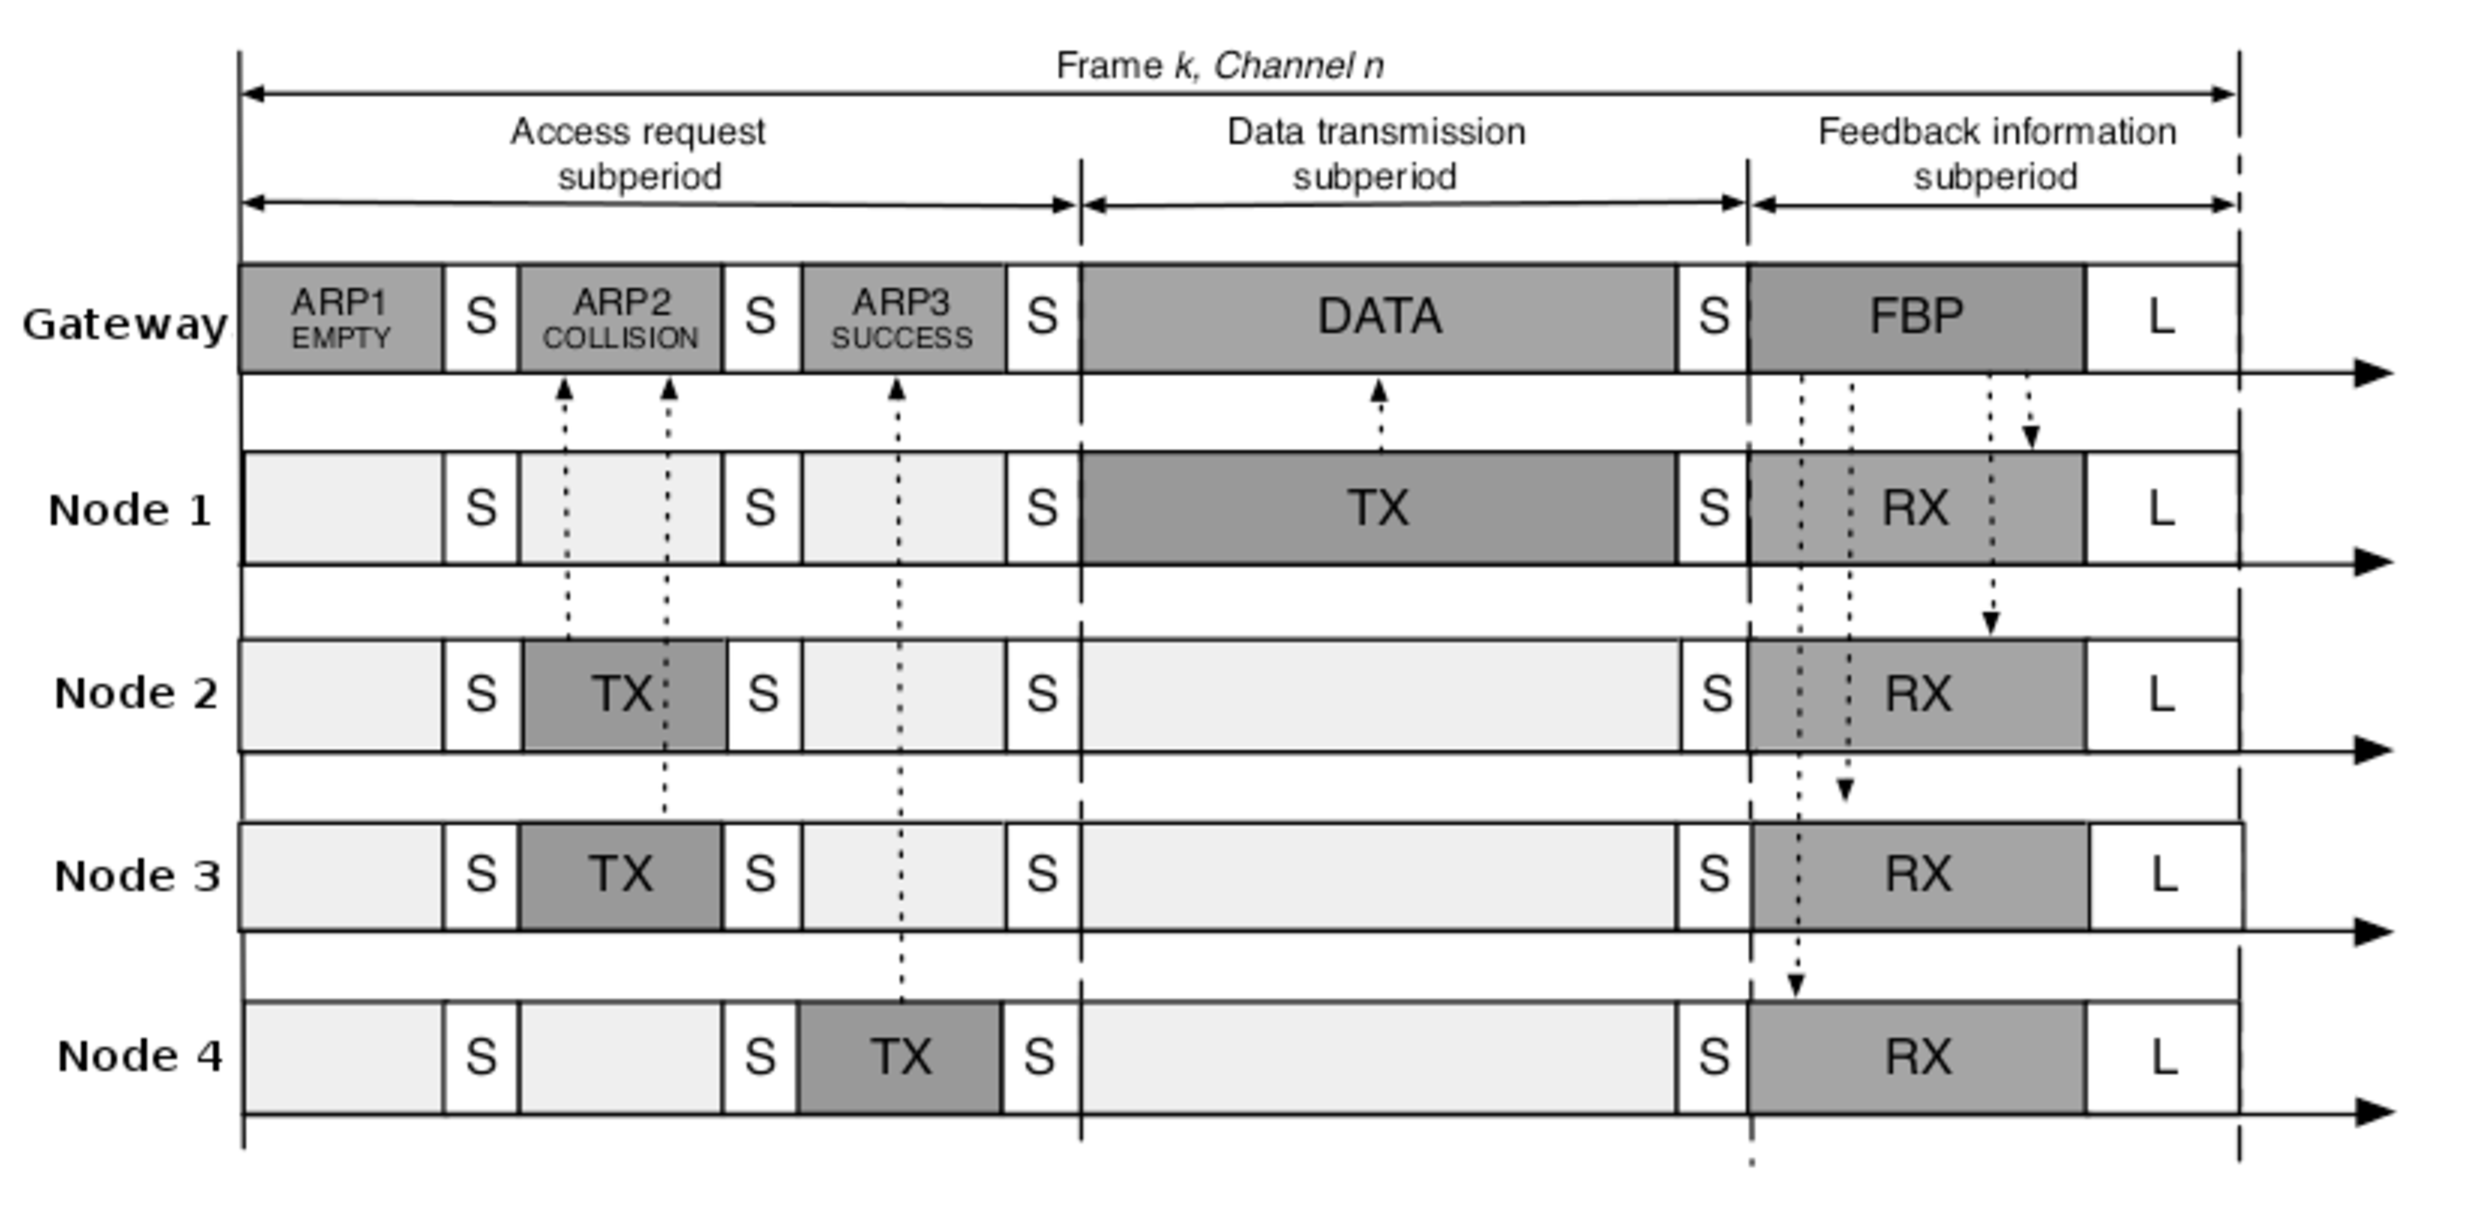
\includegraphics[width=0.75\linewidth]{07-dq}
    \caption{Distributed Queue operation.}
    \label{fig:07-dq}
\end{figure}

The DQ protocol is implemented in the $dq.c$ and $dq.h$ files in the $protocols$ folder. The implementation of DQ contains two different flavours, one for the gateway and one for the node, which are selected at compile time using a macro defined in the project configuration file ($config.h$), i.e., gateway or node. 

The DQ implementation for the gateway is responsible to transmit the FBP in the feedback sub-period at the start of every frame. The FBP contains the information regarding the global status of the different queues, i.e., CRQ and DTQ, and also the outcome of the access request and the data transmission sub-periods of the previous frame. Such information is used by all nodes in the network to determine which action to take in the current frame, i.e., remain idle, transmit in the access request sub-period or transmit in the data transmission sub-period. Then, for every slot in the access request sub-period the gateway listens to nodes transmitting an access request packet to gain access to the network. The state of the access request packet in a slot of the access request sub-period can be empty, success or collision depending on the number of nodes that have transmitted in the same slot. To determine the state of the access request packet in each slot the gateway uses the same approach as in FSA, i.e., check the RSSI (Received Signal Strength Indicator) and the CRC (Cyclic Redundancy Check)\footnote{If the RSSI is below a threshold, the gateway determines that the state of the slot is empty, e.g., no node transmitted an access request packet. If the RSSI is above a threshold and the CRC is valid the gateway determines that the state of the access request packet is success. Finally, if the RSSI is above a threshold and the CRC is not valid the gateway determines that the state  is collision, e.g., two or more nodes transmitted an access request packet in the same slot.}. Contrarily, the state of the data packet in the data transmission sub-period will be \textit{always}\footnote{The data transmit rules in DQ ensure that only one node in the network will be at the head of the DTQ at any given time. Thus, the node cannot collide with any other node during the transmission of its data packet. However, it is possible that the result of the transmission is not success due to multi-path propagation or external interference.} success. Based on the information from the slots in the access request sub-period and the data packet in the data transmission sub-period, the gateway updates the global status of the queues and creates the feedback packet that will be transmitted to the nodes in the feedback sub-period of the next frame. The process is repeated subsequently until all nodes in the network have transmitted their data packet, i.e., both the CRQ and the DTQ are empty and the status of all slots in the access request sub-period is empty.

In turn, the DQ implementation for the node is responsible to receive the FBP from the gateway in the feedback sub-period at the beginning of every frame. When a node receives the FBP from the gateway it updates the outcome of the access request and data transmission sub-periods of the previous frame and checks and updates the current status of the queues, i.e., CRQ and DTQ. Based on the global and local state of each queue the node will determine which action to take in the access request and the data transmission sub-periods of the current frame. A node can take three main actions in the access request and data transmission sub-period of each frame. If the CRQ is empty or the node holds the first position in the CRQ it will transmit an access request packet in a random slot in the access request sub-period of the current frame. The selection of the slot to transmit its access request packet in the access request sub-period is done at random following a uniform distribution, where all the slots have the same probability. Contrarily, if the node holds the first position in the DTQ the node will transmit a data packet in the data transmission sub-period of the current frame. Otherwise, i.e., the node holds none or any other position in either queue, it will remain idle until the beginning of the next frame, where it will repeat the process. After the access request and the data transmission sub-periods, the node listens to the feedback packet at the beginning of the next frame to repeat the process until it succeeds in transmitting its data packet to the gateway.

The DQ implementation has 6 main configuration parameters that determine the time length of each frame, as summarized in Table~\ref{tab:06-dq}. The first five parameters determine the length of each sub-period in a slot, i.e., $DQ\_FBP\_DURATION$, whereas the last parameter ($DQ\_SLOT\_DURATION$) represents the length of a whole DQ frame. As depicted in Figure~\ref{fig:07-dq}, a DQ slot is composed of 3~ARPs, 1~DATA, 1~FBP, 1~LIFS and 4~SIFS which, considering the current duration of a frame (364~ticks), gives an effective frame rate of 90~frames/second. Taking into account that each frame contains 127~bytes of payload, the net throughput is 91.44~kbps. Thus, taking into account that the physical layer operates at 250~kbps, DQ provides a physical layer efficiency of 36\%. Compared to FSA, as presented in Section\ref{sec:06-fsa}, the physical layer efficiency of DQ is smaller, i.e., 36\% of DQ with respect to 59.7\% of FSA (with 10 slots per frame). However, the effective throughput of FSA is smaller due to collisions caused by two nodes selecting the same slot to transmit their data packet, i.e., 36\% of DQ with respect to 22\% of FSA. Moreover, such result assumes that the gateway can know the number of nodes present in the network in advance and, thus, it can adjust the number of slots per frame to the optimal, i.e., same number of slots per frame as nodes in the network. However, such knowledge of the network cannot be assumed in most real environments and, thus, the real performance of FSA will be even worse. Finally, it is important to remark that the DQ efficiency can be increased by reducing the length of ARPs, as well as the length of LIFS and SIFS periods. However, changing the length of such parameters poses stringent requirements to maintain synchronization among nodes and, thus, it is not recommended.

% Distributed Queuing configuration parameters
\begin{table}[!it]
\centering
\begin{tabular}{|c|c|}
\hline
\textbf{PARAMETER} & \textbf{VALUE} \\ \hline
$DQ\_FBP\_DURATION$ & 44 ticks \\ \hline
$DQ\_ARP\_DURATION$ & 24 ticks \\ \hline
$DQ\_DATA\_DURATION$ & 152 ticks \\ \hline
$DQ\_SIFS\_DURATION$ & 16 ticks \\ \hline
$DQ\_LIFS\_DURATION$ & 32 ticks \\ \hline
$DQ\_SLOT\_DURATION$ & 364 ticks\\ \hline
$DQ\_ARP\_COUNT$ & 3 ARPs \\
\hline
\end{tabular}
\label{tab:06-dq}
\caption{Distributed queuing configuration parameters.}
\end{table}

Similarly to FSA, the DQ implementation has three additional configuration parameters, as described in the next listing.
\begin{itemize}
\item $DQ\_UNSYNC\_ERRORS$. Indicates the number of de-synchronization events that a node can tolerate. A de-synchronization event occurs when a node does not receive the expected packet type or the packet is not successfully received. By default, the DQ implementation tolerates up to 16 de-synchronization events before the node resets itself.
\item $DQ\_RSSI\_THRESHOLD$. Indicates the energy that is required to be present in the channel for the gateway to distinguish between successful, collision and empty data slots transmitted by Nodes. A data slot is considered successful if enough energy is present in the channel and the CRC of the data packet correct. A data slot is considered empty if the energy present in the channel is below the threshold. Finally, a data slot is considered collision if the energy present in the channel is above the threshold but a data packet has not been received or it has been received with a wrong CRC. By default, the FSA implementation uses a threshold that is set to $-85$~dBm and changing its value has several implications on the FSA performance. Setting a value higher, i.e., 80~dBm, will reduce the maximum communication range because nodes will be considered as interference. Contrarily, setting a value lower, i.e., -90~dBm, will increase the maximum communication range but lead to false collision detection. 
\item $DQ\_RADIO\_CHANNEL$. Indicates the channel at which FSA operates by default if channel hopping is not enabled. By default, channel hopping is disabled at the MAC layer (see Section~\ref{sec:06-mac}) and the FSA implementation operates in channel 26.
\end{itemize}

In addition to the configuration parameters, the DQ module also defines the data structures that are used to store information related to the operation of the protocol during the data transmission phase. In particular the DQ module defines the $dq\_vars_t$ and the $dq\_debug\_t$ data structures, as defined next.

The $dq\_vars\_t$ data structure is used to keep the variables that are used during data transmission phase using DQ by both the gateway and the node. In either case, i.e., gateway or node, there are some variables that remain unused. Thus, it would be interesting to separate this variables in to two different data structures, one for the gateway and one for the node. This would allow to reduce memory footprint and to provide a clearer approach to understand what each variable does in each case.
\begin{itemize}
\item $packet\_type$ [$dq\_packet\_type\_t$]. Type of packet, i.e., FBP, DATA or ARP.
\item $mac\_address$ [$mac\_address\_t$]. Local address of the gateway or node.
\item $seq\_number$ [$mac\_seq\_number\_t$]. Sequence number of the packet.
\item $next\_channel$ [$mac\_channel\_t$].  Channel at which DQ will operate for the next frame.

\item $arp\_count$ [$uint8\_t$]. Number of ARP slots in the access sub-period.
\item $arp\_selected$ [$uint8\_t$]. ARP selected in the access sub-period to transmit the ARP packet.
\item $arp\_transmitted$ [$uint8\_t$]. Number of ARP packets that a node has transmitted. 

\item $arp\_rssi$ [$int8\_t$]. RSSI state of the packet, i.e. above or below threshold.
\item $arp\_rssi\_threshold$ [$int8\_t$]. RSSI value to consider packets as collided.
\item $arp\_random$ [$uint8\_t$]. Value of the ARP in the current access sub-period. Currently nodes use their unique 16-bit address as the random value.

\item $arp\_total$ [$uint8\_t$]. Number of ARP packets that a node has transmitted to transmit to join the DTQ queue.
\item $crq\_wait$ [$uint8\_t$]. Position that a node holds when joining the CRQ to resolve a collision in the access sub-period.
\item $dtq\_wait$ [$uint8\_t$]. Position that a node holds when joining the DTQ to transmit a data packet in the data sub-period.

\item $unsync\_error$ [$uint8\_t$]. Number of unsynchronization errors.

\item $crq\_local$ [$dq\_crq\_length\_t$]. Local length of the CRQ queue.
\item $pcrq\_local$ [$dq\_crq\_length\_t$]. Local position in the CRQ queue.
\item $dtq\_local$ [$dq\_dtq\_length\_t$]. Local length of the DTQ queue.
\item $pdtq\_local$ [$dq\_dtq\_length\_t$]. Local position in the DTQ queue.

\item $arp1\_state$ [$dq\_arp\_state\_t$]. State of ARP\#1 in the access sub-period, i.e., empty, success or collision.
\item $arp1\_random$ [$dq\_arp\_random\_t$]. Value of the ARP\# 1 in the access sub-period. Currently nodes use their unique 16-bit address as the random value.
\item $arp1\_rssi$ [$dq\_arp\_rssi\_t$]. RSSI state of ARP\#1 in the access sub-period, i.e., above or below the threshold.
\item $arp2\_state$ [$dq\_arp\_state\_t$]. State of ARP\#2 in the access sub-period, i.e., empty, success or collision.
\item $arp2\_random$ [$dq\_arp\_random\_t$]. Value of the ARP\#2 in the access sub-period. Currently nodes use their unique 16-bit address as the random value.
\item $arp2\_rssi$ [$dq\_arp\_rssi\_t$]. RSSI state of ARP\#2 in the access sub-period, i.e., above or below the threshold.
\item $arp3\_state$ [$dq\_arp\_state\_t$]. State of ARP\#3 in the access sub-period, i.e., empty, success or collision.
\item $arp3\_random$ [$dq\_arp\_random\_t$]. Value of the ARP\#3 in the access sub-period. Currently nodes use their unique 16-bit address as the random value.
\item $arp3\_rssi$ [$dq\_arp\_rssi\_t$]. RSSI state of the ARP\#3 in the access sub-period, i.e., above or below the threshold.

\item $data\_state$ [$dq\_data\_state\_t$]. State of the data packet in the data sub-period, i.e., empty, success or collision.
\item $data\_address$ [$mac\_address\_t$]. Address of the node that transmitted its data packet in the data sub-period.

\item $crq\_global$ [$dq\_crq\_length\_t$]. Global length of the CRQ queue.
\item $dtq\_global$ [$dq\_dtq\_length\_t$]. Global length of the DTQ queue.
\end{itemize}

The $dq\_debug\_t$ data structure is used to keep debug information related to the DQ operation. The $dq\_debug\_t$ is packed and is transmitted through the serial line to the computer at the end of every data sub-period. Such information is used by the application to create the statistics of the data transmission phase.
\begin{itemize}
\item $mac\_type$ [$mac\_type\_t$]. MAC type (DQ).

\item $arp1\_state$ [$dq\_arp\_state\_t$]. State of ARP\#1, i.e., empty, success or collision.
\item $arp2\_state$ [$dq\_arp\_state\_t$]. State of ARP\#2, i.e., empty, success or collision.
\item $arp3\_state$ [$dq\_arp\_state\_t$]. State of ARP\#3, i.e., empty, success or collision.
\item $data\_state$ [$dq\_data\_state\_t$]. State of DATA, i.e., empty, success or collision.

\item $arp1\_rssi$ [$int8\_t$]. RSSI state of ARP\#1 in the access sub-period, i.e., above or below the threshold.
\item $arp2\_rssi$ [$int8\_t$]. RSSI state of ARP\#2 in the access sub-period, i.e., above or below the threshold.
\item $arp3\_rssi$ [$int8\_t$]. RSSI state of ARP\#3 in the access sub-period, i.e., above or below the threshold.

\item $arp\_total$ [$uint8\_t$]. Number of ARP packets that a node has transmitted to join the DTQ queue to transmit a data packet.
\item $crq\_wait$ [$uint8\_t$]. Position that a node holds when joining the CRQ to resolve a collision in the access sub-period.
\item $dtq\_wait$ [$int8\_t$]. Position that a node holds when joining the DTQ to transmit a data packet in the data sub-period.

\item $arp1\_random$ [$dq\_arp\_random\_t$]. Address of the node in ARP\#1. The address will be empty ($0x0000$) if the ARP was empty or collision.
\item $arp2\_random$ [$dq\_arp\_random\_t$]. Address of the node in ARP\#2. The address will be empty ($0x0000$) if the ARP was empty or collision.
\item $arp3\_random$ [$dq\_arp\_random\_t$]. Address of the node in ARP\#3. The address will be empty ($0x0000$) if the ARP was empty or collision.
\item $data\_address$ [$mac\_address\_t$]. Address of the node in DATA. The address will be empty ($0x0000$) if the DATA packet was empty or collision.

\item $crq\_local$ [$dq\_crq\_length\_t$]. Local length of the CRQ queue.
\item $crq\_global$ [$dq\_crq\_length\_t$]. Global length of the CRQ queue.
\item $pcrq\_local$ [$dq\_crq\_length\_t$]. Pointer to the position in the CRQ queue.

\item $dtq\_local$ [$dq\_dtq\_length\_t$]. Local length of the DTQ queue.
\item $dtq\_global$ [$dq\_dtq\_length\_t$]. Global length of the DTQ queue.
\item $pdtq\_local$ [$dq\_dtq\_length\_t$]. Pointer to the position in the DTQ queue.
\end{itemize}

In addition to the timing parameters, the DQ implementation also determines the structure for the DQ packets: $dq\_fbp\_t$ for the feedback packet, $dq\_data\_t$ for the data packet and $dq\_arp\_t$ for the access request packet.

The $dq\_fbp\_t$ packet is transmitted by the gateway in the feedback sub-period of each frame. The $dq\_fbp\_t$ packet is 24~bytes long and contains the information described in the following listing. Considering the SHR (5~bytes) at the physical layer and the FCS (2~bytes) at the data-link layer, the $dq\_fbp\_t$ packet is 27~bytes long and takes 0.864~ms (28,31~ticks) to be completely transmitted.
\begin{itemize}
\item $mac\_type$ [$uint8\_t$]. MAC type (DQ).
\item $packet\_type$ [$uint8\_t$]. Packet type (FBP).
\item $source$ [$uint16\_t$]. Address of the gateway transmitting the data packet.
\item $destination$ [$uint16\_t$]. Broadcast ($0xFFFF$) since all nodes within communication range are expected to receive feedback packets.
\item $seq\_number$ [$uint16\_t$]. Sequence number of the current frame to allow nodes ensure that they are correctly synchronized.
\item $arp1\_state$ [$uint8\_t$]. State of ARP\#1, i.e., empty, success or collision.
\item $arp1\_random$ [$uint16\_t$]. Value of the ARP\# 1 in the access sub-period. Currently nodes use their unique 16-bit address as the random value.
\item $arp2\_state$ [$uint8\_t$]. State of ARP\#2, i.e., empty, success or collision.
\item $arp2\_random$ [$uint16\_t$]. Value of the ARP\#2 in the access sub-period. Currently nodes use their unique 16-bit address as the random value.
\item $arp3\_state$ [$uint8\_t$]. State of ARP\#3, i.e., empty, success or collision.
\item $arp3\_random$ [$uint16\_t$]. Value of the ARP\#3 in the access sub-period. Currently nodes use their unique 16-bit address as the random value.
\item $data\_state$ [$uint8\_t$]. State of DATA, i.e., empty, success or collision.
\item $crq\_global$ [$uint16\_t$]. Global length of the CRQ queue.
\item $dtq\_global$ [$uint16\_t$]. Global length of the DTQ queue.
\item $arp\_count$ [$uint8\_t$]. Number of ARPs in the access sub-period in the next frame. This could enable to dynamically adjust the number of number of ARPs in the access sub-period based on collision estimation algorithms.
\item $next\_channel$ [$uint8\_t$]. Channel at which the gateway will operate for the next frame. This could enable to do channel hopping to combat multi-path propagation and external interference.
\end{itemize}

The $dq\_data\_t$ packet is transmitted by the node at the head of the DTQ in the data sub-period. The $dq\_data\_t$ packet is 125~bytes long and contains the information described in the following listing. Considering the SHR (5~bytes) at the physical layer and the FCS (2~bytes) at the data-link layer, the $dq\_data\_t$ packet is 128~bytes long and takes 4.096~ms (134.25~ticks) to be completely transmitted.
\begin{itemize}
\item $mac\_type$ [$uint8\_t$]. MAC type (DQ).
\item $packet\_type$ [$uint8\_t$]. Packet type (DATA).
\item $source$ [$uint16\_t$]. Address of the node transmitting the data packet.
\item $destination$ [$uint16\_t$]. Address of the gateway that will receive the data packet.
\item $arp\_total$ [$uint8\_t$]. Number of ARP packets that a node has transmitted to join the DTQ queue to transmit a data packet.
\item $crq\_wait$ [$uint8\_t$]. Position that a node holds when joining the CRQ to resolve a collision in the access sub-period.
\item $dtq\_wait$ [$uint8\_t$]. Position that a node holds when joining the DTQ to transmit a data packet in the data sub-period.
\item $data$ [$uint8\_t$]. Remaining bytes of the packet payload (116~bytes) that can be used to transport data from the node to the gateway.
\end{itemize}

The $dq\_arp\_t$ packet is transmitted by the the nodes at that want to join the DTQ to transmit a data packet in the access sub-period. The $dq\_arp\_t$ packet is 4~bytes long and contains the information described in the following listing. Considering the SHR (5~bytes) at the physical layer and the FCS (2~bytes) at the data-link layer, the $dq\_arp\_t$ packet is 7~bytes long and takes 0.224~ms (7.34~ticks) to be completely transmitted.
\begin{itemize}
\item $mac\_type$ [$uint8\_t$]. MAC type (DQ).
\item $packet\_type$ [$uint8\_t$]. Packet type (ARP).
\item $random\_number$ [$uint16\_t$]. Random value for the ARP. Currently nodes use their unique 16-bit address as the random value.
\end{itemize}

The DQ module also defines the following public functions that are common for both the gateway and the node implementation.
\begin{itemize}
\item $dq\_init$ Initializes the $dq\_vars$ and the $dq\_debug\_serial$ variables and sets the local address of the node by calling the $ueee\_addr\_get\_eui16$ function. It is called from the MAC module $mac\_init$ function during the initialization phase.
\item $dq\_start$ Starts the execution of DQ at the beginning of the data transmission phase by pushing the $dq\_fbp\_init$ function to the scheduler.
\end{itemize}

The DQ module also defines the following private functions that implement the gateway state machine of the DQ protocol. The compilation of such functions is protected by the $MAC\_DEVICE$ macro, that is, the functions are only compiled if the $MAC\_DEVICE$ is equal to $MAC\_GATEWAY$ as defined in the $config.h$ file in each project.
\begin{itemize}
\item $dq\_fbp\_init$. Executed at the beginning of each frame. Obtains an entry from the $packet\_buffer$ module and prepares the paypload of the feedback packet based on the information available in the $dq\_vars$. After that, it registers the radio transmit interrupts, puts the feedback packet to the radio transceiver and transmits it. Finally, it creates a timeout for the duration of the feedback packet using the $virtual\_timer$ module that will execute the $dq\_fbp\_done$ function when it expires.
\item $dq\_fbp\_tx\_init$. Callback from the radio transceiver to indicate that the feedback packet is now being transmitted.
\item $dq\_fbp\_tx\_done$. Callback from the radio transceiver to indicate that the feedback packet has been successfully transmitted.
\item $dq\_fbp\_done$. Executed when the timeout configured from the $dq\_fbp\_init$ functions expires. Puts the radio transceiver back to idle mode and releases the entry from the $packet\_buffer$ module. Then, it transmits the $dq\_debug\_serial$ variable through the serial port using the $serial\_push\_message$ function. Finally, it creates a timeout using the $virtual\_timer$ module that will execute the $dq\_ack\_init$ function when it expires.

\item $dq\_arp\_init$. Executed when the timeout configured from $dq\_fbp\_done$ expires. Puts the radio transceiver in receive mode to get an access request packet from the nodes. Finally, it computes the ticks remaining until the middle of the access request packet and creates a timeout using the $virtual\_timer$ module that will execute the $dq\_arp\_rx\_rssi$ function when it expires.
\item $dq\_arp\_rx\_init$. Callback from the radio transceiver to indicate that a packet is now being received.
\item $dq\_arp\_rx\_rssi$. Callback from the $virtual\_timer$ module to indicate that it is the middle of the access request packet. It samples the RSSI value and then computes the ticks remaining until the end of the access request packet. Finally, it creates a timeout using the $virtual\_timer$ module that will execute the $dq\_arp\_done$ function when it expires.
\item $dq\_arp\_rx\_done$. Callback from the radio transceiver to indicate that a packet has been successfully received. It obtains an entry from the $packet\_buffer$ module and copies the payload from the radio transceiver.
\item $dq\_arp\_done$. Executed when the timeout configured from $dq\_arp\_rx\_rssi$ expires. Puts the radio transceiver back to idle mode. It first, parses the state of the current access request packet and determines if it was empty, successful or collision using the CRC and the RSSI sample. Finally, it releases the entry from the $packet\_buffer$ module and creates a timeout using the $virtual\_timer$ module. If this is the last access request packet, the timeout will execute the $dq\_data\_init$ function to start the data sub-period to let the node at the head of the DTQ transmit its data packet. Otherwise, the timeout will execute the $dq\_arp\_init$ function again to receive another access request packet.

\item $dq\_data\_init$. Executed when the timeout configured from $dq\_arp\_done$ expires. Puts the radio transceiver in receive mode to get a data packet from the nodes. Finally, it computes the ticks remaining until the middle of data packet and creates a timeout using the $virtual\_timer$ module that will execute the $dq\_data\_done$ function when it expires.
\item $dq\_data\_rx\_init$. Callback from the radio transceiver to indicate that a packet is now being received.
\item $dq\_data\_rx\_done$. Callback from the radio transceiver to indicate that a packet has been successfully received. It obtains an entry from the $packet\_buffer$ module and copies the payload from the radio transceiver.
\item $dq\_data\_done$. Executed when the timeout configured from $dq\_data\_init$ expires. Puts the radio transceiver back to idle mode and releases the entry from the $packet\_buffer$ module. It processes the received packet and determines if it was empty, successful or collision using the CRC and the RSSI sample. With such information it fills in the $dq\_debug$ variable using the $dq\_vars\_log$ function and transmits it using the through the serial port using the $serial\_push\_message$ function. Finally, it creates a timeout using the $virtual\_timer$ module that will execute the $dq\_fbp\_init$ function when it expires.

\item $dq\_vars\_reset$. Resets the contents of the $dq\_vars$ variable.
\item $dq\_vars\_log$. Copies the $dq\_vars$ variables that will be transmitted through the serial port to the $dq\_debug\_serial$ variable.
\end{itemize}

Similarly, the DQ module defines the following private functions that implement the node state machine of the DQ protocol. The compilation of such functions is protected by the $MAC\_DEVICE$ macro, that is, the functions are only compiled if the $MAC\_DEVICE$ is equal to $MAC\_NODE$ as defined in the $config.h$ file in each project.
\begin{itemize}
\item $dq\_fbp\_init$. Executed at the beginning of each frame. Resets the $dq\_vars$ variables and prepares to receive a feedback packet from the gateway. Finally, it computes the maximum number of ticks remaining until the end of the feedback packet and creates a timeout using the $virtual\_timer$ module that will execute the $dq\_fbp\_done$ function.
\item $dq\_fbp\_rx\_init$. Callback from the radio transceiver to indicate that a packet is now being received. It stops the current timeout and creates a new timeout using the exact number of ticks remaining until the expected end of the feedback packet. The function assumes that it is indeed a feedback packet, so it is possible to know the exact number of ticks that remain.
\item $dq\_fbp\_rx\_done$. Callback from the radio transceiver to indicate that a packet has been received. It obtains an entry from the $packet\_buffer$ module and copies the payload from the radio transceiver. It then checks that if payload is valid and contains a feedback packet. If so, it updates the DQ variables with the $dq\_vars\_update$ function.

\item $dq\_fbp\_done$. Executed when the timeout configured from either the $dq\_fbp\_init$ or the $dq\_fbp\_rx\_init$ functions expires. It puts the radio transceiver back to idle mode and releases the entry from the $packet\_buffer$ module. Then it checks if the packet received is a valid feedback packet. If so, it indicates that it is synchronized with the gateway and applies the DQ rules by executing the $dq\_qdr\_rules$ function. Then it checks if the CRQ and DTQ lengths are consistent by executing the $dq\_qdr\_check$ function. If the queues are inconsistent, it notifies the MAC module that it has lost synchronization and calculates the ticks remaining until the start of the feedback packet and creates a timeout using the $virtual\_timer$ module that will execute the $dq\_fbp\_init$ function when it expires. If the queues are consistent, it first updates the CRQ and DTQ length and positions using the $dq\_qdr\_update$ function and updates the DQ statistics. Afterwards, it checks if it can transmit an access request packet by executing the $dq\_rtr\_check$ function. If so, it decides which access request slot it will use by executing the $dq\_arp\_vars\_set$ and then it calculates the ticks remaining until the start of the selected access request packet and creates a timeout using the $virtual\_timer$ module that will execute the $dq\_arp\_init$ function when it expires. Alternatively, it checks if it can transmit a data packet by executing the $dq\_dtr\_check$ function. If so, it resets the variables related to the access request packet, calculates the ticks remaining until the start of the data packet and creates a timeout using the $virtual\_timer$ module that will execute the $dq\_data\_init$ function when it expires. Finally, if it is not allowed to transmit an access request packet or a data packet, i.e., because it is waiting in either the CRQ or the DTQ queue, it calculates the ticks remaining until the start of the feedback packet and creates a timeout using the $virtual\_timer$ module that will execute the $dq\_fbp\_init$ function when it expires.

\item $dq\_arp\_init$. Executed when the timeout configured from $dq\_fbp\_done$ or $dq\_arp\_done$ expires. If the current access request packet is the one that has been selected to transmit, it obtains an entry from the $packet\_buffer$ module and fills it in with the access request packet payload. After that, it loads the packet to the radio transceiver and puts the radio transceiver in transmit mode. Finally it creates a timeout for the duration of the data packet using the $virtual\_timer$ module that will execute the $dq\_arp\_arp\_done$ function when it expires.
\item $dq\_arp\_tx\_init$. Callback from the radio transceiver to indicate that a packet is now being transmitted.
\item $dq\_arp\_tx\_done$. Callback from the radio transceiver to indicate that a packet has been successfully transmitted.
\item $dq\_arp\_done$. Executed when the timeout configured from $dq\_arp\_init$ expires. Puts the radio transceiver back to idle mode and releases the entry from the $packet\_buffer$ module. Finally, it increments the counter of elapsed access request packets. If this is the last access request packet it calculates the ticks remaining until the start of the feedback packet and creates a timeout using the $virtual\_timer$ module that will execute the $dq\_fbp\_init$ function when it expires. If this is the selected access request packet it calculates the ticks remaining until the start of the data packet and creates a timeout using the $virtual\_timer$ module that will execute the $dq\_data\_init$ function when it expires. Otherwise, if this is not the selected or the last access request packet it calculates the ticks remaining until the start of the next access request packet and creates a timeout using the $virtual\_timer$ module that will execute the $dq\_arp\_init$ function when it expires.

\item $dq\_data\_init$. Executed when the timeout configured from $dq\_arp\_done$ expires. It obtains an entry from the $packet\_buffer$ module,  fills it in with the data payload and resets the related counters. After that, it loads the packet to the radio transceiver and puts the radio transceiver in transmit mode. Finally, it creates a timeout for the duration of the data packet using the $virtual\_timer$ module that will execute the $dq\_data\_done$ function when it expires.
\item $dq\_data\_tx\_init$. Callback from the radio transceiver to indicate that the data packet is now being transmitted.
\item $dq\_data\_tx\_done$. Callback from the radio transceiver to indicate that the data packet has been successfully transmitted.
\item $dq\_data\_done$. Executed when the timeout configured from $dq\_data\_init$ expires. Puts the radio transceiver back to idle mode and releases the entry from the $packet\_buffer$ module. Finally, it computes the ticks remaining until the start of the feedback packet and creates a timeout using the $virtual\_timer$ module that will execute the $dq\_fbp\_init$ function when it expires.

\item $dq\_arp\_vars\_set$. Sets the value of the $dq\_vars$ variable with the appropriate information.
\item $dq\_arp\_vars\_reset$. Resets the value of the $dq\_vars$ variable.
\item $dq\_data\_vars\_reset$. Sets the value of the $dq\_vars$ variable with the appropriate information.

\item $dq\_vars\_update$. Sets the value of the $dq\_vars$ variable with the information from the feedback packet.
\item $dq\_dtr\_check$. Checks the data transmit rules to determine if a node can transmit in the data sub-period.
\item $dq\_rtr\_check$. Checks the access transmit rules to determine if a node can transmit in the access request sub-period.
\item $dq\_qdr\_check$. Checks if the length of the CRQ and the DTQ are consistent with the ones received in the feedback packet.
\item $dq\_qdr\_update$. Updates the position in the CRQ and the DTQ based on the information received in the feedback packet.
\end{itemize}

Last but not least, the DQ module defines the following private functions that is common for both the gateway and the node implementation.
\begin{itemize}
\item $dq\_qdr\_rules$. Updates the status of the $dq\_vars$ variables based on the information received on the feedback packet.
\end{itemize}

Finally, it is important to mention that, contrarily to FSA, DQ does not have a limit in the time that nodes can maintain synchronization due to clock drift. This is because the current implementation of DQ forces all nodes to listen to all FBP that are transmitted by the gateway. Such packets allow nodes to compensate for the clock drift and keep synchronized with the gateway. However, this comes at the cost of an increased energy expenditure. Since nodes have to listen to all FBPs regardless of the state of the CRQ and DTQ queues, the energy consumption is increased. In that sense, it would be possible to change the implementation so that nodes only listen to enough FBPs to maintain synchronization. However, such mode of operation is currently not implemented.
